\myparagraph{Purpose}
Any special user can manage its profile from \textit{Data4Help} web site, in particular:
\begin{itemize}
  \item The special user can change some of its informations: its legal address, its billing address, its corporate e-mail address and the sector in which it operates;
  \item The special user can change all the data regarding its legal representative;
  \item The special user can see the data it has required and paied until this moment;
  \item The special user can see the payments it hasn't paied yet;
  \item The special user can change the preferred payment method;
  \item The special user can change its password;
  \item The special user can delete its profile.
\end{itemize}

\myparagraph{Scenario 1}
The executive director of PincoPallo SPA had a serious fight with the legal representative of his company, and he decided to fire him a week ago. Now that he has find a new legal he wants to change the data stored in his \textit{Data4Help} profile. He accesses to \textit{Data4Help} web site from his personal pc, he logs in with the company profile and he goes in "\textit{Edit profile}" area. Now he inserts all the information about the new legal in the matching fields and then clicks on the "\textit{Submit changes}" button.

\myparagraph{Scenario 2}
AlphaAnalisi SPA wants to change the preferred payment method due to changes in its internal organization. It opens \textit{Data4Help} main page, logs in and goes in its "\textit{Edit profile}" area. It clicks on the "\textit{Change payment method}" button and selects the new preferred method. Finally it clicks on the "\textit{Submit changes}" button.

\myparagraph{Use Case}
The \textit{Special Profile Visualization} use case is analyzed in Table \ref{table:specialProfileVisualizationTable}. \\
The \textit{Modify Personal Information} use case is analyzed in Table \ref{table:modifyPersonalInformationTable}. \\
The \textit{Change Password} use case is analyzed in Table \ref{table:changePassowrdTable}. \\
The \textit{Delete Profile} use case is analyzed in Table \ref{table:deleteProfileTable}. \\

\myparagraph{Mockup}
The \textit{Special Profile Visualization} mockup is shown in Figure \ref{img:specialProfileVisualizationMockup}.

\myparagraph{Functional requirements}
\begin{enumerate}
  \item The system must let the special user view its personal profile at anytime;
  \item The system must let the special user upload/change its personal information at anytime;
  \item The system must let the special user change its password only if the old one has been inserted correctly;
  \item The system must not let the special user change its password if the new one has not been inserted correctly twice;
  \item The system must let the special user delete its profile at anytime;
  \item The system must require to confirm a deleting request;
  \item The system must not delete a profile if the choice isn't confirmed by the special user;
  \item The system must let the special user leave the editing profile process at anytime;
\end{enumerate}

\begin{center}
\begin{table}
\begin{tabular}{ | l | p{0.75\linewidth} | }
  \hline
    Actor & \textbf{Special user} \\ \hline
    Goal & \textbf{[G.3]} \\ \hline
    Input Condition & A \textbf{Special user} wants to view its profile\\ \hline
    Event Flow & \begin{minipage}[t]{0.7\textwidth}
      \begin{enumerate}
        \item The \textbf{Special user } opens \textit{Data4Help} web site;
        \item The \textbf{Special user} logs in;
        \item The \textbf{Special user} accesses to its personal area;
        \item The system shows to the \textbf{Special user} its "\textit{Edit profile}" area and the buttons to move to "\textit{Past Request}" area and "\textit{Pending Requests}" area.
      \end{enumerate}
    \smallskip
  \end{minipage} \\ \hline
  Output Condition & The \textbf{Special user} views its profile withss all the related information\\ \hline
  Exceptions & None \\ \hline
\end{tabular}
\caption{\textit{Special profile visualization} use case}
\label{table:specialProfileVisualizationTable}
\end{table}
\end{center}

\begin{figure}
\begin{center}
  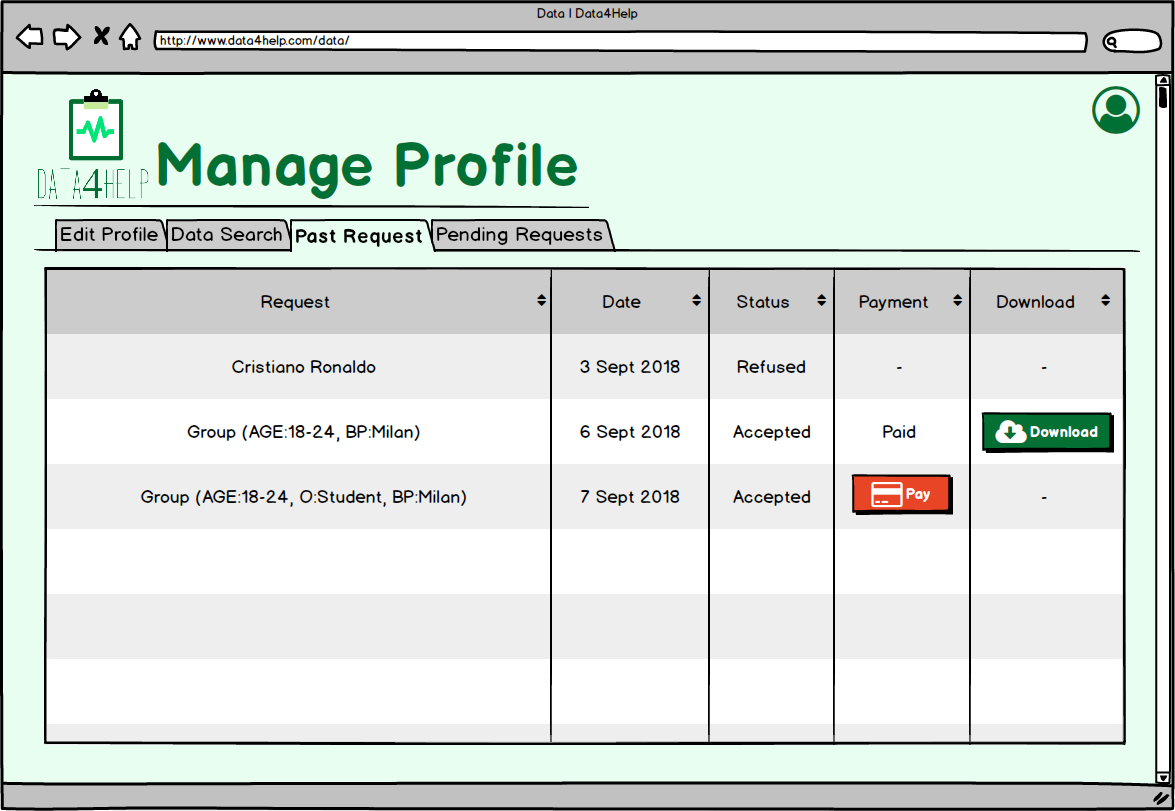
\includegraphics[width=\textwidth]{img/mockup/Searched.png}
  \hspace{0.05\linewidth}
  \centering
  \caption{\textit{Special Profile Visualization} mockup}
  \label{img:specialProfileVisualizationMockup}
\end{center}
\end{figure}
